
\subsection{OT Calibration}

\begin{figure}[h]
  \centering
  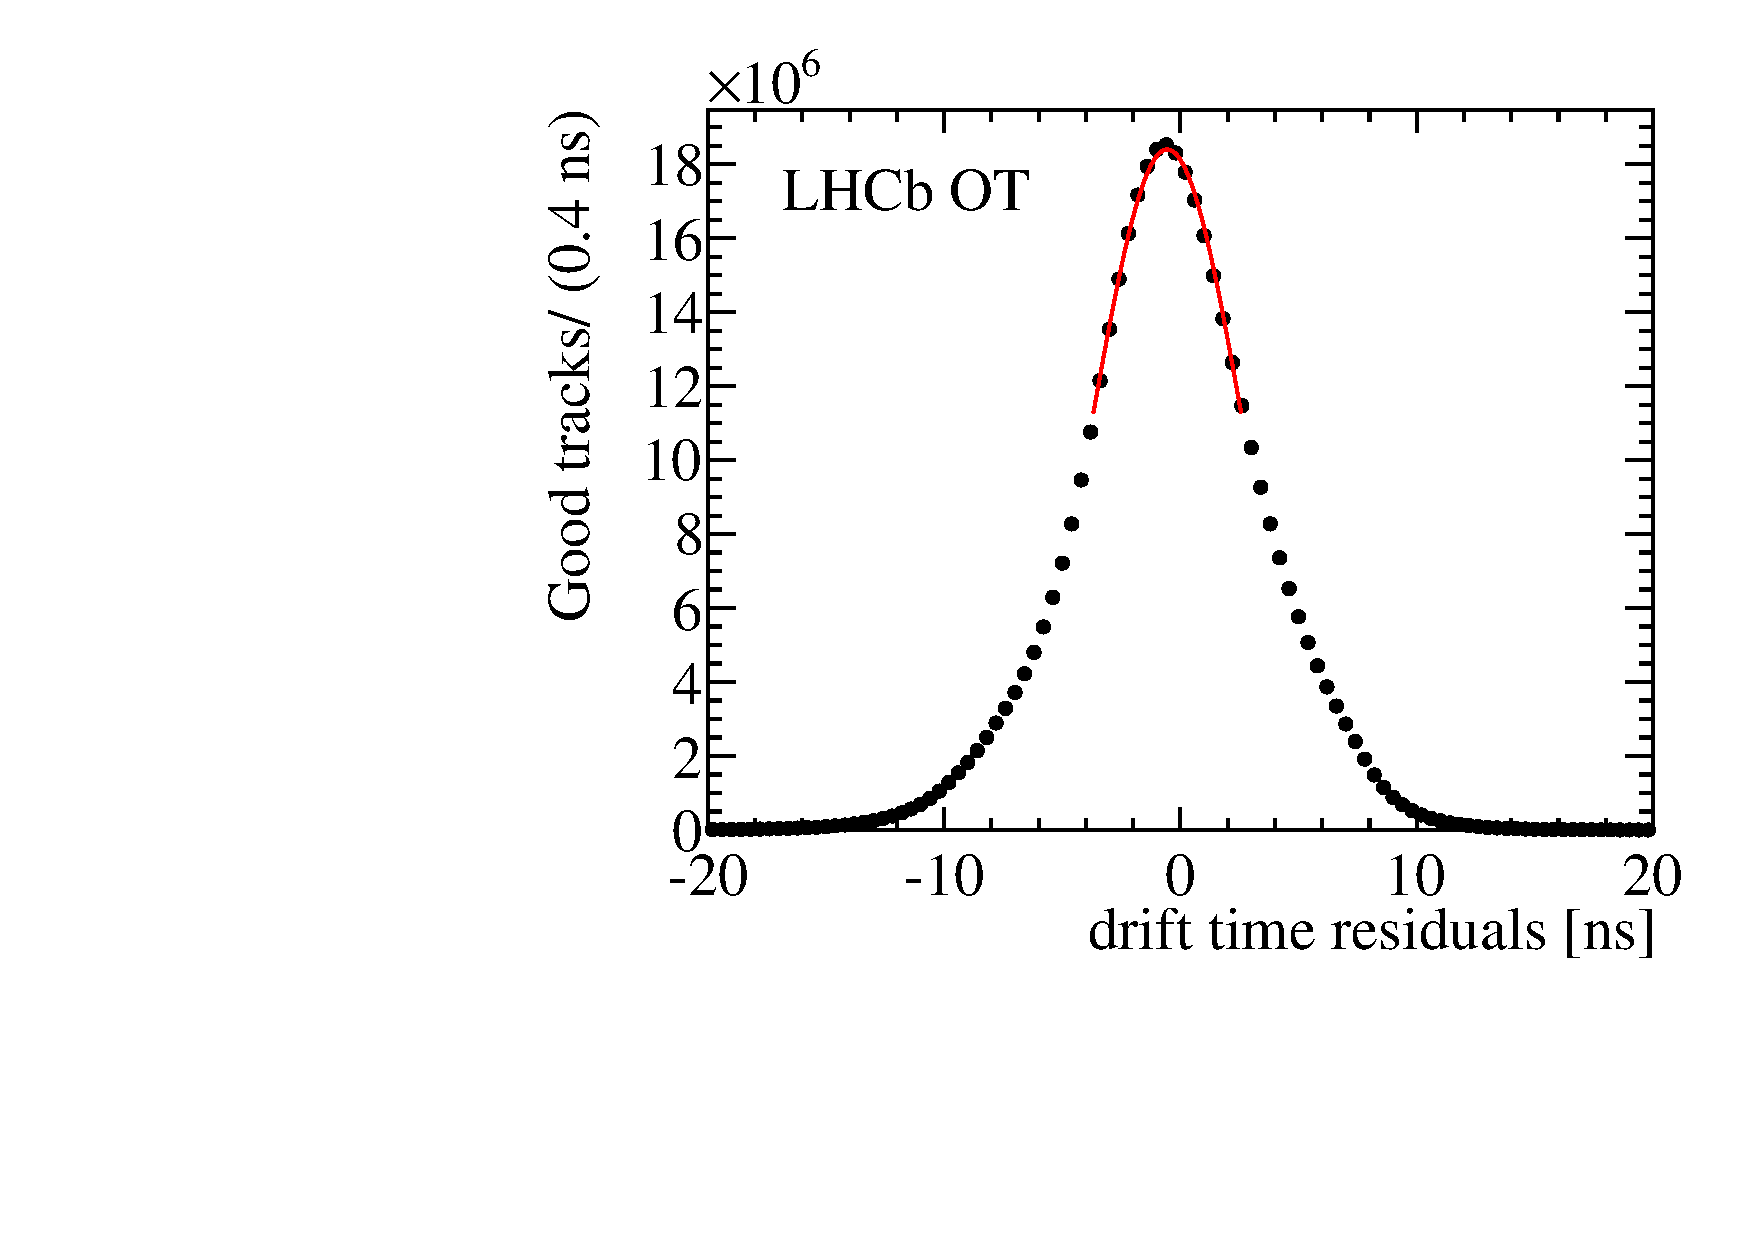
\includegraphics[width=8cm]{../figures/OT_fit}
  \caption{Fit to the distribution of the drift-time residuals of Outer Tracker
    hits, used to estimate the global time offset between the collision time and
    the LHC clock.}
  \label{fig:OT_calib}
\end{figure}

The LHCb Outer Tracker (OT) \cite{LHCb-DP-2013-003} is a detector consisting of
gas-filled straws with a 5 mm pitch. The time difference between a bunch
crossing and the measurement of a signal in one of the straws,
$t_{\text{meas}}$, consists of several compenents as expressed by:
\begin{equation}
  t_{\text{meas}} = t_0 + t_{\text{flight}} + t_{\text{prop}} + t_{\text{drift}},
\end{equation}
where $t_0$ is the time delay caused by the readout electronics,
$t_{\text{flight}}$ is the time-of-flight of the charged particle that caused
the signal, $t_{\text{prop}}$ is the time required for the signal to propagate
along the wire to the readout electronics, and $t_{\text{drift}}$ the drift-time
of electrons in the gas.

While the $t_0$ time delay is different for each read-out board of the OT, it
can be written as the sum of a average, detector-wide, offset and a per-board
offset. As the per-board offsets are a property of the electronics, they are
expected to change very little. The global offset changes more frequently as a
result of, for example, drift of the arrival time of the LHC clock to which the
readout is synchronised. To correct for these global clock changes, a
near-realtime analysis is performed to calibrate it.

Data accepted by the HLT1 stage of the HLT is sent to a small farm running of
$O(50)$ of the LHCb reconstruction application, Brunel. Good quality tracks
that traverse the Velo and OT are selected and the expected drift-times of hits
in the OT are calculated from the track parameters. The residual differences
between the expected and measured drift-times are entered into a histogram and a
fit of a Gaussian function to the central part of the resulting distribution is
performed to extract the global offset. An example of such a fit it shown in
\cref{fig:OT_calib}.

Data is collected in LHCb in periods of up to an hour long, called runs. The
calibration is performed at most once per run once a distribution of drift-time
residuals of sufficient size has been obtained; fifty thousand entries are
typically sufficient. The task that performs the calibration waits for the
distribution of drift-time residuals to be made available to it, which occurs
approximately every fifteen minutes, and at the end of a run. The calibration is
then performed and if the difference with the last known best calibration is
larger than a threshold, the new calibration is saved and automatically
propagated to all tasks running online at the start of the next run; it is also
inserted into the database used by tasks running
offline. \Cref{fig:OT_calib_time} shows the values of the global time offset
obtained during July and August of 2015.

\begin{figure}[h]
  \centering
  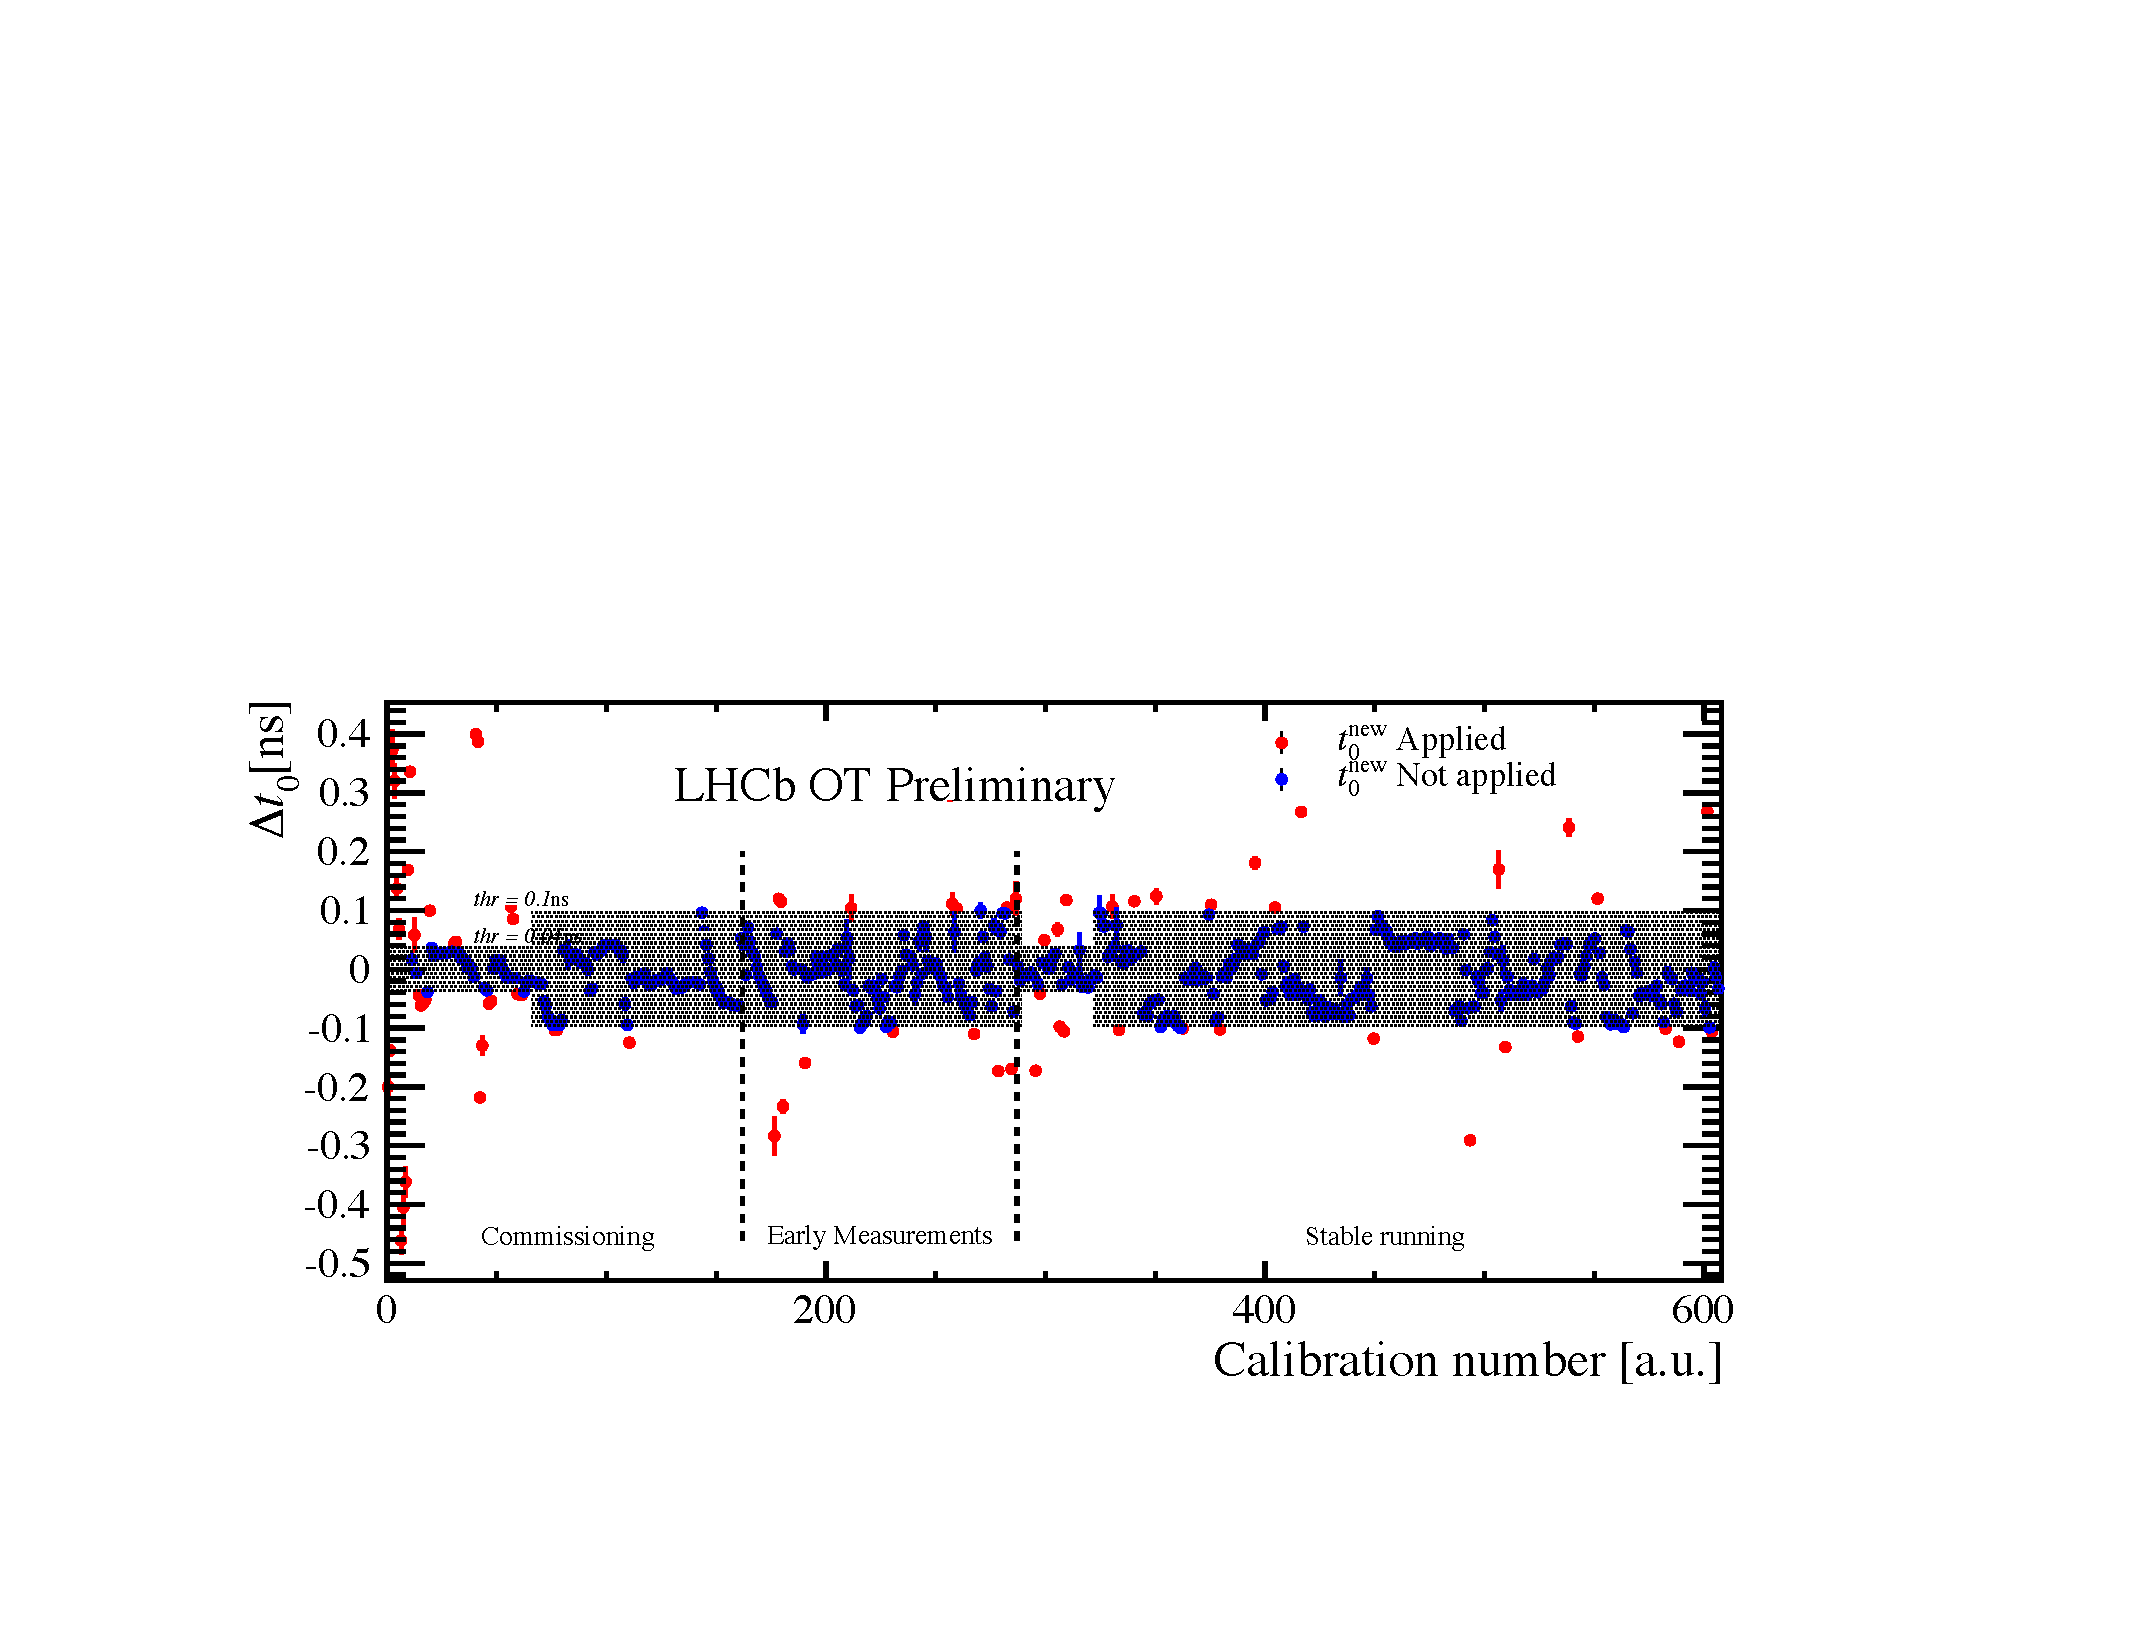
\includegraphics[width=10cm]{../figures/OTt0calibration2015}
  \caption{Global $t_0$ values obtained by the calibration task over time. Red
    points indicate values that were above threshold and therefore propagated to
    online and offline tasks and databases.}
  \label{fig:OT_calib_time}
\end{figure}
